\section{Inheritance}
\subsection{Inheritance and Subtyping}
\begin{mytitle}[Inheritance vs. Subtyping] Subtyping expresses classification, Inheritance is a means of code reuse. Inheritance is usually coupled with subtyping. Example for subtyping without inheritance: Java Interfaces. Example for inheritance without subtyping: C++ private inheritance. Subclassing = Subtyping + Inheritance.
\end{mytitle}
\begin{mytitle}[Sets and Bounded Sets]\hfill\\
\lstset{language=Java}
\begin{minipage}[t]{0.5\textwidth}
\begin{lstlisting}
class Set{
    int size;
    
    void add(Object o){
        //add o 
    }
    
    boolean contains(Object o){
        ...
    }
}
\end{lstlisting}
\end{minipage}
\begin{minipage}[t]{0.5\textwidth}
\begin{lstlisting}
class BoundedSet{
    int size;
    int capacity;
    
    void add(Object o){
        //add o if there is space
    }
    
    boolean contains(Object o){
        ...
    }
}
\end{lstlisting}
\end{minipage}
BoundedSet is not a behavioral subtype of Set, but Set is also not a behavioral subtype of BoundedSet. We would still like to reuse the code. General answer: Subtyping dominates inheritance!
\begin{itemize}
    \item Aggregation: BoundedSet uses Set, method calls are delegated to Set. Here it works, but there are other examples, where we need subtyping.
    \item Creating New Objects: Let BoundedSet be a subclass of Set. In add, just return a new larger BoundedSet with all the elements, if it wouldn't fit in the old one. This makes the set not really bounded anymore, so this is not what users of BoundedSet want.
    \item Weak Superclass Contracts: Just have the weakest contracts in a new superclass, and make the two classes behavioral subtypes. Could even introduce static contracts, which specify a given method implementation. Dynamically-bound calls use the standard contract, while statically-bound calls use a combination of static and standard contracts. With those, this is good design.
    \item Inheritance w/o Subtyping: Like private/protected inheritance in C++ or non-conforming inheritance in Eiffel.
\end{itemize}
\end{mytitle}

\subsection{Dynamic Method Binding}
\begin{mytitle}[Method Binding]\hfill
\begin{itemize}
    \item Static binding: At compile time, a method declaration is selected for each call based on the static type of the receiver expression. Examples: C++ (because of performance), C\#(because of versioning). This is one of the most fundamental differences between C\# and Java.
    \item Dynamic binding: At run time, a method declaration is selected for each call based on the dynamic type of the receiver object. This enables specialization and subtype polymorphism. However we have an performance overhead of method look-up at run-time and it makes it harder to evolve code without breaking subclasses. Examples: Eiffel, Java, Scala, all dynamically-typed languages.
\end{itemize}
\end{mytitle}
\begin{mytitle}[Fragile Baseclass Scenario] Subclasses can be affected by changes to superclasses. How should we apply inheritance to make our code robust against revisions of superclasses?
\begin{itemize}
    \item Subclass: Using inheritance, rely on interface documentation not implementation. Override all methods that could break invariants. Avoid specializing classes that are expected to be changed often.
    \item Superclass: Do not change calls to dynamically-bound methods.
    \item In C++ methods are bound statically by default. Potential overrides must be declared as either override or new (default). This prevents accidental overriding. 
\end{itemize}
\end{mytitle}
\begin{mytitle}[Overloading]\hfill
\begin{itemize}
    \item In Java, overloading resolution chooses the most specific method declaration from all methods that are available. So adding methods to a superclass may affect clients of the subclass.
    \item In C++, overloading resolution chooses the most specific method declaration in the class of the receiver, then in the superclass etc. Adding methods to a superclass does not affect overloading resolution.
\end{itemize}
\end{mytitle}
\begin{mytitle}[Binary Methods] Binary methods take a receiver and one explicit argument. Often behaviour should be specialized depending on the dynamic types of both arguments. But covariant parameter types are not statically type-safe.
\begin{itemize}
    \item Explicit Type Tests: Type test and conditional for specialization based on dynamic type of explicit type argument. Problems: tedious to write, code is not extensible, requires type cast.
    \item Double Invocation (Visitor Pattern): Additional dynamically-bound call for specialization based on dynamic type of explicit argument. This does a flip of the arguments: First we have t1.calls(t2) and then t2.calls(t1), so for each of the parameters of the initial binary method, there is a dynamically bound call where the parameter is the receiver. Problems: even more tedious to write, requires modification of superclass. So this is only applicable if one has the whole subclass hierarchy under control. 
    \item Overloading plus Dynamic: Cast parameters to dynamic. Dynamic resolution depends on dynamic types of both arguments. Problems: not entirely type-safe, overhead for run-time checks. Also we do not know what it returns, so we might run into a run-time error.
    \item Multiple Dispatch: Some research languages allow method calls to be bound based on the dynamic type of several arguments. Problems: Performance overhead of method look-up at run-time, extra requirements are needed to ensure there is a unique best method for every call.
\end{itemize}
\end{mytitle}

\subsection{Multiple Inheritance}
\begin{mytitle}[Simulating Multiple Inheritance] In Java and C\#, we can simulate multiple inheritance via aggregation and delegation. 
\end{mytitle}
\begin{mytitle}[Problems of Multiple Inheritance] \hfill
\begin{itemize}
    \item Ambiguities: Superclasses may contain fields and methods with identical names and signatures. Which version should be available in the subclass? 
    \item Repeated inheritance (diamond of death): A class may inherit from a superclass more than once. How many copies of the superclass members are there? How are the superclass fields initialized?
\end{itemize}
\end{mytitle}
\begin{mytitle}[Ambiguity]\hfill
\begin{itemize}
    \item Explicit Selection: Ambiguity is resolved by client. Clients need to know implementation details. C++ does it like this with the scope operator.
    \item Merging Methods: Related inherited methods can be merged into one overriding method. This does not work for fields and unrelated methods. The subclass should provide both methods, but with different names.
    \item Renaming: Inherited methods can be renamed. Dynamic binding takes renaming into account. This is the cleanest solution and is used by Eiffel and C++/CLI, a dialect of C++.
\end{itemize}
\end{mytitle}
\begin{mytitle}[Repeated Inheritance] How many address fields should PhDStudent have? How are they initialized?
\lstset{language=C++}
\begin{lstlisting}
    class Person{
        Address address;
        ...
    };
    class Student: public Person{
        ...
    };
    class Assistant: public Person{
        ...
    };
    class PhDStudent: public Student, public Assistant{
        ...
    };
\end{lstlisting}
\begin{minipage}{0.4\textwidth}
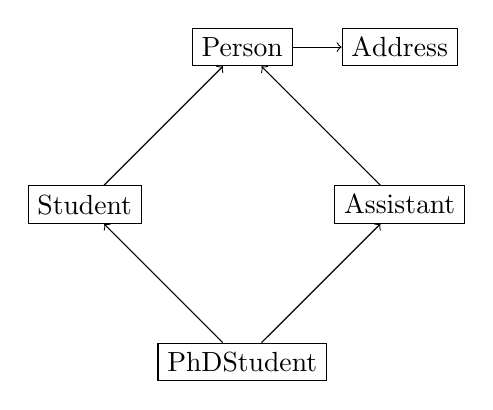
\begin{tikzpicture}
    \node[draw] (a) at (0,0) {PhDStudent};
    \node[draw] (b) at (-2,2) {Student};
    \node[draw] (c) at (2,2) {Assistant};
    \node[draw] (d) at (0,4) {Person};
    \node[draw] (e) at (2,4) {Address};
    \draw[->] (a) -- (b);
    \draw[->] (b) -- (d);
    \draw[->] (a) -- (c);
    \draw[->] (c) -- (d);
    \draw[->] (d) -- (e);
\end{tikzpicture}\hfill\\
\begin{center}
Virtual inheritance: \\
Default in Eiffel. \\
Virtual inheritance in C++.
\end{center}
\end{minipage}
\begin{minipage}{0.6\textwidth}
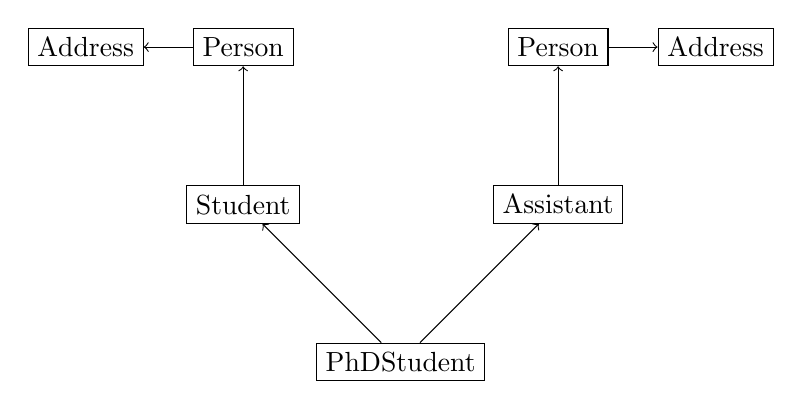
\begin{tikzpicture}
    \node[draw] (a) at (0,0) {PhDStudent};
    \node[draw] (b) at (-2,2) {Student};
    \node[draw] (c) at (2,2) {Assistant};
    \node[draw] (d) at (-2,4) {Person};
    \node[draw] (f) at (2,4) {Person};
    \node[draw] (e) at (-4,4) {Address};
    \node[draw] (g) at (4,4) {Address};
    \draw[->] (a) -- (b);
    \draw[->] (b) -- (d);
    \draw[->] (a) -- (c);
    \draw[->] (c) -- (f);
    \draw[->] (d) -- (e);
    \draw[->] (f) -- (g);
\end{tikzpicture}\hfill\\
\begin{center}
Non-Virtual Inheritance:\\
Renaming field in Eiffel. \\
Default in C++.
\end{center}
\end{minipage}
\end{mytitle}
\begin{mytitle}[Inheritance and Object Initialization] Normally, superclass fields are initialized before subclass fields. This call can also be implicit like in Java. This helps preventing use of uninitialized fields. Order is typically implemented via mandatory call of superclass constructor at the beginning of each constructor. 
\begin{itemize}
    \item Non-Virtual Inheritance: With non-virtual inheritance, there are two copies of the superclass field. Superclass constructor is called twice to initialize both copies. 
    \item Virtual Inheritance: With virtual inheritance, there is only one copy of the superclass field. Who gets to call the superclass constructor? If both do it, we get a number of problems. First, we could have two different arguments to the constructor. Second, final fields would get initialized twice and thirdly, there could be side-effects in the constructor. The solution in C++ is that the smallest subclass (e.g. PhDStudent in the example) needs to call the constructor of the virtual superclass directly. So programmers need foresight and constructors cannot rely on the virtual superclass constructors they call. Eiffel does not force constructors to call superclass constructors. So subclasses have to initialized inherited fields. Subclasses also need to understand the implementation of the whole superclass tree. The policy is to always call the superclass "init" method, then constructors of repeated superclasses get called twice. This can be problematic.
\end{itemize}
\end{mytitle}
\begin{mytitle}[Summary]\hfill\\
\begin{center}
    \begin{tabular}{R{0.4\textwidth}|L{0.4\textwidth}}
       \textbf{Pros}  & \textbf{Cons} \\
       \hline
        Increases expressiveness & Ambiguity resolution\\
        Avoids overhead of delegation pattern & Repeated inheritance\\
         & Complicated!
    \end{tabular}
\end{center}
\end{mytitle}

\subsection{Linearization}
\begin{mytitle}[Mixins and Traits] Mixins and traits provide a form of reuse. Methods and state can be mixed into various classes. Main applications are to make thin interfaces thick and stackable specifications. To avoid multiple inheritance among classes, the class must be a subclass of its traits' superclasses. Each trait defines an abstract type. Extending or mixing-in a trait introduces a subtype relation. Traits can be mixed-in upon class declaration or upon class instantiation. Languages that support mixins or traits: Python, Ruby, Scala, Squeak Smalltalk.
\end{mytitle}
\begin{mytitle}[Scala Trait Example]\hfill\\
\lstset{language=Scala}
\begin{minipage}[t]{0.55\textwidth}
\begin{lstlisting}
class Cell{
    var value: Int = 0
    
    def put(v: Int) = {value = v}
    def get: Int = value
}
trait Backup extends Cell{
    var backup: Int = 0
    
    override def put(v: Int) = {
        backup = value
        super.put(v)
    }
    def undo = {super.put(backup)}
}
\end{lstlisting}
\end{minipage}
\begin{minipage}[t]{0.5\textwidth}
\begin{lstlisting}
object Main1{
    def main(args: Array[String]){
        val a = new Cell with Backup
        a.put(5)
        a.put(3)
        a.undo
    }
}

class FancyCell extends Cell with Backup{
    ...
}
\end{lstlisting}
\end{minipage}
\end{mytitle}
\begin{mytitle}[Ambiguity Resolution] Ambiguity is resolved by merging. If two inherited methods override a common superclass method, merging is not required. 
\end{mytitle}
\begin{mytitle}[Linearization] The key concept to understand the semantics of Scala traits: bring types in a linear order. Define overriding and super-calls according to this order. For a class or template Sub extends Super with T1 ... with Tn, we have the linearization 
$$L(Sub) = Sub, L(Tn) \bullet \hdots \bullet L(T1)\bullet L(Super)$$ 
with 
$$\epsilon\ \bullet\ B = B \qquad (A,B)\ \bullet\ (C) = \left\{
    \begin{tabular}{l l}
        $A, (B\ \bullet\ C)$ & $if A \notin C$\\
        $A\ \bullet\ C$ & otherwise
    \end{tabular}\right.$$
So every class shows up exactly once in the linearization. Subclass inherits only one copy of a repeated superclass. Like Eiffel and virtual inheritance in C++. Classes and traits are initialized in the reverse linear order. Each constructor is called exactly once. Arguments to superclass constructors are supplied by the immediately preceding class (not trait) in the linearization order. 
\end{mytitle}
\begin{mytitle}[How to do Linearization]\hfill
\begin{enumerate}
    \item Put main class first.
    \item For the rest of the classes and traits, go from right to left.
    \item For each of those, do the first two points recursively
    \item Go from right to left and ignore all that we have already.
\end{enumerate}
Example: 
\lstset{language=Scala}
\begin{lstlisting}
class A { print("A") }
class B extends A { print("B") }
trait C { print("C") }
trait D extends C { print("D") }
trait E { print("E") }
trait F extends E with C { print("F") }
class X extends B with F with D { print("X") }

new X
\end{lstlisting}
\begin{enumerate}
    \item Put main class first: 
        $$X$$
    \item For the rest of the classes and traits, go from right to left: 
        $$X \bullet D \bullet F \bullet B$$
    \item For each of those, do the first two points recursively:
        $$X \bullet (D,C) \bullet (F, C, E) \bullet (B, A)$$
    \item Go from right to left and ignore all that we have already: 
        $$X, D, F, C, E, B, A$$
\end{enumerate}
Note that the command \texttt{new X} would print the reversed linearization order when run.
\end{mytitle}
\begin{mytitle}[Stackable Specializations] With traits, specializations can be combined in flexible ways. With multiple inheritance, methods of repeated superclasses are called twice. Example
\begin{minipage}{0.5\textwidth}
\lstset{language=Scala}
\begin{lstlisting}
class Queue{
    def put(x: Data){...}
}
trait Timer extends Queue{
    override def put (x: Data){
        x.SetTime(...);
        super.put(x);
    }
}
trait Filter extends Queue{
    override def put(x: Data){
        if(x.Time > ...);
        super.put(x);
    }
}
class SensorData extends Queue 
    with Filter with Timer{}
\end{lstlisting}
\end{minipage}
\begin{minipage}{0.5\textwidth}
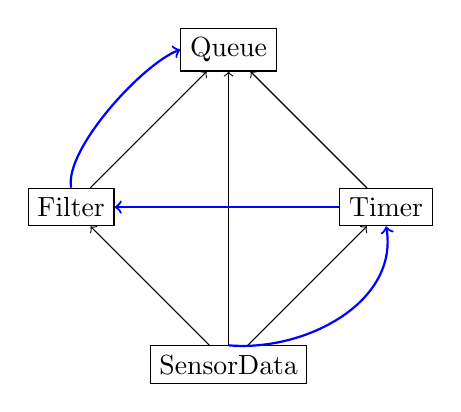
\begin{tikzpicture}
    \node[draw] (a) at (0,0) {SensorData};
    \node[draw] (b) at (2,2) {Timer};
    \node[draw] (c) at (-2,2) {Filter};
    \node[draw] (d) at (0,4) {Queue};
    
    \draw[->] (a) -- (b);
    \draw[->] (a) -- (c);
    \draw[->] (a) -- (d);
    \draw[->] (b) -- (d);
    \draw[->] (c) -- (d);
    
    \draw[->, thick, color=blue] (a.north) to [out=-5,in=-80] (b.south);
    \draw[<-,thick, color=blue] (c.east) -- (b.west);
    \draw[->,thick, color=blue,distance=0.5cm] (c.north) to [out=100,in=200] (d.west);
\end{tikzpicture}
\end{minipage}
In Eiffel or C++, we would either only get one specialization or put the object into the queue twice. But we need to derive the order of the traits, so we need the code of them. 
\end{mytitle}
\begin{mytitle}[Reasoning about Traits] Traits are very dynamic, which complicates state reasoning. Traits do not know which methods they override. Traits do not know where super-calls are bound to. Also two classes with the same traits but in another order have the same type. This is a mistake!
\end{mytitle}